\Section{Нули регулярной функции. Теорема единственности}

Пусть \(f(z)\) регулярна в \(z_0\). Тогда существует окрестность этой точки \(B_R(z_0)\), в которой
\(f(z)\) представима в виде \(f(z) = \sum\limits_{k = 0}^\infty c_k (z-z_0)^k\).

\begin{definition}
    \(z_0\)~--- нуль функции \(f\), если \(f(z_0) = 0\), то есть \(c_0 = 0\). \(z_0\)~--- нуль 
    порядка \(n\), если \(c_n \ne 0\), но \(\forall k < n \rightarrow c_k = 0\). Если все 
    \(c_k = 0\), то \(z_0\)~--- нуль бесконечного порядка.
\end{definition}

\begin{example}
    \(\sin{z^3} = z^3 - \dfrac{z^9}{6} + \dots\). Нуль \(z = 0\) является нулём порядка 3 (также 
    можно обозначать \(\mathbb{H}_3\)).
\end{example}

\begin{statement}\label{20:isolated_zeros}
    \textbf{(Изолированность нулей конечного порядка).} Пусть \(z_0\)~--- нуль порядка \(n\)
    регулярной функции \(f\). Тогда \(\exists \mathring{B}_{R_1}(z_0)\colon f(z) \ne 0 \, \forall z 
    \in \mathring{B}_{R_1}(z_0)\).
\end{statement}

\begin{proof}
    По определению имеем разложение в ряд Тейлора в некоторой окрестности \(B_R(z_0)\): \(f(z) = 
    c_n(z-z_0)^n + c_{n+1}(z-z_0)^{n+1} + \dots = (z-z_0)^n(c_n + c_{n+1} (z-z_0) + \dots)\). В этом
    представлении \(c_n \ne 0\). Ряд в скобках сходится в \(B_R(z_0)\), поэтому сумма этого ряда 
    непрерывна в этой окрестности, а значит \(\exists B_{R_1}(z_0) \, (R_1 \le R)\) в которой эта
    сумма не равна нулю. Тогда \(f(z) \ne 0 \, \forall z \in \mathring{B}_{R_1}(z_0)\).
\end{proof}

\begin{statement}
    \textbf{(Теорема единственности).} Пусть:
    \begin{enumerate}[wide=20pt, label=\arabic*., itemsep=0ex]
        \item \(f(z)\) регулярна в области \(G \subset \Co\);
        \item \(\forall z \in E \subset G \rightarrow f(z) = 0\);
        \item \(\exists z_0 \in G\) предельная для множества \(E\).
    \end{enumerate}
    Тогда \(f(z) \equiv 0\) на области \(G\).
\end{statement}

\begin{proof}
    \textbf{Шаг 1.} Так как \(z_0\) предельная для \(E\), то \(\exists \{z_n\}\)~--- 
    последовательность попарно различных точек, такая что: \(z_n \rightarrow z_0, \, n \rightarrow
    \infty\). В силу непрерывности \(f(z)\) в \(z_0\) имеем: \(f(z_0) = \lim\limits_{n \rightarrow 
    \infty} f(z_n) = 0\), то есть \(z_0\) неизолированный нуль регулярной функции \(f\), поэтому 
    \(f(z) \equiv 0\) в любом кргуе \(B_R(z_0) \subset G\).

    \textbf{Шаг 2.} Зафиксируем \(z_1 \in G\), \(z_1 \ne z_0\). Покажем, что \(f(z_1) = 0\).
    Предположим противное, то есть \(f(z_1) \ne 0\). Тогда в силу непрерывности \(f(z)\) существует
    \(B_{R_1}(z_1) \colon f(z) \ne 0\). Определим кривую \(\gamma \colon z = z(t), \, t \in [a,b],
    \, z(a) = z_0, \, z(b) = z_1\).

    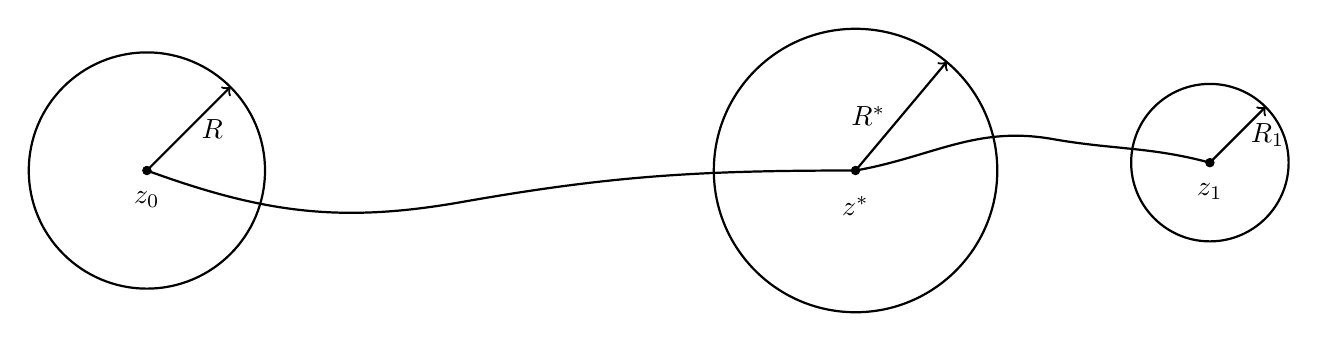
\begin{tikzpicture}
    % Левый круг: центр z0, радиус R
    \draw[thick] (0,0) circle (1.5);
    \filldraw (0,0) circle (1.5pt) node[below=4pt] {$z_0$};
    \draw[thick, ->] (0,0) -- (45:1.5) node[midway, right=1pt] {$R$};

    % Кривая от z0 к z*
    \draw[thick] (0,0) to[out=-20, in=190] (4, -0.4) to[out=10, in=180] (9,0);

    % Средний круг: обычная окружность, сплошная точка z*, радиус R*
    \begin{scope}[shift={(9,0)}]
        \draw[thick] (0,0) circle (1.8);
        \filldraw (0,0) circle (1.5pt) node[below=6pt] {$z^*$};
        \draw[thick, ->] (0,0) -- (50:1.8) node[midway, left=2pt] {$R^*$};
    \end{scope}

    % Кривая от z* к z1
    \draw[thick] (9,0) to[out=10, in=170] (11.5, 0.4) to[out=-10, in=165] (13.5, 0.1);

    % Правый круг: центр z1, радиус R1
    \begin{scope}[shift={(13.5, 0.1)}]
        \draw[thick] (0,0) circle (1.0);
        \filldraw (0,0) circle (1.5pt) node[below=4pt] {$z_1$};
        \draw[thick, ->] (0,0) -- (45:1.0) node[midway, right=1pt] {$R_1$};
    \end{scope}
    \end{tikzpicture}

    Пусть \(t^* = \inf\limits_{t \in [a,b]}\{t\ \colon f(z(t)) \ne 0\}\). Пусть \(z^* = z(t^*)\).
    Тогда \(\exists B_{R^*}(z^*) \subset G\). В силу определения \(t^*\) \(\forall t < t^* 
    \rightarrow f(z(t)) = 0\). В \(z^*\) \(f(z^*) = \lim\limits_{t \rightarrow t^* - 0} f(z(t)) =0\)
    в силу непрерывности сложной функции \(f(z(t))\), а значит \(z^*\)~--- неизолированный нуль 
    регулярной функции \(f\), тогда по утверждению \ref{20:isolated_zeros} это нуль бесконечного
    порядка, а значит \(f(z) \equiv 0\) в \(B_{R^*}(z^*)\).

    В силу непрерывности \(z(t)\) имеем: \(\exists \delta > 0\colon \forall t \in (t^*-\delta,
    t^*+\delta) \rightarrow |z(t) - z^*| < R^*\), то есть \(z(t) \in B_{R^*}(z^*)\). Но тогда 
    \(f(z(t)) = 0\) при \(a \le t \le t^* + \delta\). Это противоречит определению \(t^*\).
\end{proof}

\begin{corollary}
    Пусть:
    \begin{enumerate}[wide=20pt, label=\arabic*., itemsep=0ex]
        \item \(f(z), g(z)\) регулярны в области \(G \subset \Co\);
        \item \(\forall z \in E \subset G \rightarrow f(z) = g(z)\);
        \item \(\exists z_0 \in G\) предельная для множества \(E\).
    \end{enumerate}
    Тогда \(f(z) \equiv g(z)\) на области \(G\).
\end{corollary}

\begin{corollary}
    Любая элементарная функция имеет не более одного регулярного продолжения из \(\R\) в \(\Co\).
\end{corollary}


\Section{Локально равномерно сходящиеся функциональные последовательности и ряды}

\begin{definition}
    Пусть последовательность функций \(\{f_n(z)\}\) определена в области \(G \subset \Co\). Говорим,
    что \(f_n(z)\) стремится к \(f(z)\) локально равномерно (ЛР) в \(G\), если для любого компакта 
    \(D \subset G\) верно \(f_n \mathrel{\mathop{\rightrightarrows}\limits_{D}} f\). Ряд 
    \(\sum\limits_{n=0}^\infty f_n(z)\) сходится к \(S(z)\) локально равномерно в \(G\), если к
    \(S(z)\) сходится локально равномерно последовательность его частичных сумм.
\end{definition}

\begin{example}
    \(\sum\limits_{n = 0}^\infty z^n\) сходится в \(|z| < 1\) локально равномерно, но не равномерно.
    Последнее следует из того, что даже на действительной оси этот ряд не сходится на \((-1; 1)\).
\end{example}

\begin{note}
    Если ряд \(\sum\limits_{n = 0}^\infty c_n(z-z_0)^n\) сходится в \(|z-z_0| < R\), то эта 
    сходимость локально равномерна.
\end{note}

\begin{proof}
    (Доказательство данного утверждения было дано как упражнение). Пусть \(D \subset B_R(z_0)\)~--- 
    произвольный компакт. Так как \(D\) замкнут и ограничен, а функция расстояния \(|z - z_0|\) 
    непрерывна на \(D\), по теореме Вейерштрасса достигается максимум:
    \[
        r = \max\limits_{z \in D} |z - z_0|.
    \]
    Так как \(D \subset B_R(z_0)\), для всех \(z \in D\) выполнено \(|z - z_0| < R\), откуда 
    \(r < R\).сЗафиксируем точку \(z_1 = z_0 + \rho\), выбрав \(\rho\) так, что \(r < \rho < R\). 
    Так как \(|z_1 - z_0| = \rho < R\), числовой ряд \(\sum\limits_{n=0}^\infty c_n (z_1 - z_0)^n\)
    сходится.

    Тогда по теореме Абеля степенной ряд сходится равномерно в замкнутом круге
    \(\overline{B}_r(z_0) = \{z \in \Co \colon |z - z_0| \le r\}\). Поскольку \(D \subset 
    \overline{B}_r(z_0)\),ряд сходится равномерно и на компакте \(D\). В силу произвольности выбора 
    компакта \(D\) сходимость в \(|z - z_0| < R\) локально равномерна.
\end{proof}

\begin{statement}\label{21:1_th_veiershtrassa}
    \textbf{(Первая теорема Вейерштрасса).} Пусть \(f_n(z)\) регулярны в области \(G\) и на ней 
    \(f_n(z)\) стремится к \(f(z)\) локально равномерно. Тогда \(f(z)\) регулярна в \(G\).
\end{statement}

\begin{proof}
    Зафиксируем произвольный открытый круг \(K \subset G\). Пусть \(\gamma \subset K\)~--- 
    произвольный КНД контур. По интегральной теореме Коши для односвязной области \(K\) для любого
    \(n\) верно \(\int\limits_\gamma f_n(z) dz = 0\). Так как \(\gamma\) компакт, то по условию
    \(f_n \mathrel{\mathop{\rightrightarrows}\limits_{\gamma}} f\), а значит \(\int\limits_\gamma
    f(z) dz = \lim\limits_{n \rightarrow \infty} \int\limits_\gamma f_n(z) dz = 
    \lim\limits_{n \rightarrow \infty} 0 = 0\). Тогда по теореме Мореры \(f(z)\) регулярна в \(K\) в
    силу произвольности \(\gamma\). Так как \(K\)~--- произвольный, то \(f\) регулярна в \(G\).
\end{proof}

\begin{statement}
    \textbf{(2 теорема Вейерштрасса).} В условиях утверждения \ref{21:1_th_veiershtrassa} для
    любого натурального \(m\) верно, что \(f_n^{(m)}\) стремится к \(f^{(m)}\) локально равномерно
    на \(G\).
\end{statement}

\begin{proof}
    Зафиксируем \(m, \epsilon > 0, z_0 \in G, R > 0\colon \overline{B_R(z_0)} \subset G\). По 
    интегральным формулам Коши для производных для любого \(z\) из \(B_R(z_0)\) выполняется:

    \[f_n^{(m)}(z) = \dfrac{m!}{2 \pi i} \int\limits_{|\zeta - z_0| = R} \dfrac{f_n(\zeta) d\zeta}
    {(\zeta - z)^{m+1}},\]
    \[f^{(m)}(z) = \dfrac{m!}{2 \pi i} \int\limits_{|\zeta - z_0| = R} \dfrac{f(\zeta) d\zeta}
    {(\zeta - z)^{m+1}}.\]

    Зафиксируем \(R_1 \in (0, R)\). Тогда для \(z \in B_{R_1}(z_0)\) имеем \(|f_n^{(m)} - f^{(m)}|
    = \left|\dfrac{m!}{2 \pi i} \int\limits_{|\zeta - z_0| = R} \dfrac{(f_n(\zeta) - f(\zeta)) 
    d\zeta}{(\zeta - z)^{m+1}}\right| \le \dfrac{m!}{2\pi} \max\limits_{|\zeta - z_0| = R} |f_n
    (\zeta) - f(\zeta)| \dfrac{2\pi R}{(R-R_1)^{m+1}} \le \dfrac{m! \cdot R}{(R-R_1)^{m+1}} \cdot 
    \epsilon\) при всех достаточно больших \(n\), так как \(f_n(\zeta) 
    \mathrel{\mathop{\rightrightarrows}\limits_{|\zeta - z_0| = R}} f(\zeta)\). Итак, \(f_n^{(m)} 
    \mathrel{\mathop{\rightrightarrows}\limits_{B_{R_1}(z_0)}} f^{(m)}\). Это доказывает, что 
    \(\forall z_0 \in G \, \exists B_{R_1}(z_0)\colon f_n^{(m)}
    \mathrel{\mathop{\rightrightarrows}\limits_{B_{R_1}(z_0)}} f^{(m)}\).

    Пусть \(G \subset G\) произвольный компакт. Для любого \(z\) из \(D\) найдём \(B(z)\) на которой
    \(f_n^{(m)} \mathrel{\mathop{\rightrightarrows}\limits_{B(z)}} f^{(m)}\). Тогда все в 
    совокупности \(B(z)\)~--- открытое покрытие \(D\). По лемме Гейне-Бореля из этого покрытия можно
    выбрать конечное подпокрытие \(D \subset B(z_1) \cup B(z_2) \cup \dots \cup B(z_N)\). Так как 
    \(f_n^{(m)} \mathrel{\mathop{\rightrightarrows}\limits_{B(z_i)}} f^{(m)}\) для любого 
    \(i \le N\), то и на их объединении сходимость равномерна, а значит и на \(D\) она равномерна.
    В силу произвольности \(D\) утверждение доказано.
\end{proof}

\begin{note}
    \textbf{(Формулировки 1 и 2 теорем Вейерштрасса для рядов).} Если ряд регулярных в области \(G\)
    функций \(f_n(z)\) сходится локально равномерно в \(G\) к \(S(z)\), то:
    \begin{enumerate}[wide=20pt, label=\arabic*., itemsep=0ex]
        \item \(S(z)\) регулярна в \(G\);
        \item \(S^{(m)}(z) = \sum\limits_{n = 0}^\infty f_n^{(m)}(z)\);
    \end{enumerate}
\end{note}


\Section{Ряд Лорана}

Будем обозначать ряд \(\sum\limits_{n = -\infty}^{+\infty} c_m(z-z_0)^m = \sum\limits_{n = -\infty}
^{-1}\dots + \sum\limits_{n = 0}^{+\infty}\dots = N_1 + N_2\) как \((*)\). \(z_0\)~--- центр 
разложения. Ряд \((*)\) сходится в точке \(z\), если сходятся оба ряда \(N_1\) и \(N_2\), где 
\(N_2\)~--- степенной ряд, а \(N_1\)~--- результат подстановки \(w = \dfrac{1}{z-z_0}\) в степенной 
ряд \(\sum\limits_{m = 1}^{+\infty}c_{-m}w^m\), который будем обозначать как \((**)\). Пусть 
\(r\)~--- радиус сходимости ряда \(N_2\), а \(\rho\)~--- радиус сходимости ряда \((**)\). Если 
\(\rho = 0\), то \(N_1\) не определён ни при каком \(z\). Если \(\rho > 0\), то ряд \(N_1\) сходится
при \(|z-z_0| > \dfrac{1}{\rho}\).

\begin{definition}
    Если \(\dfrac{1}{\rho} < r\), то \(\dfrac{1}{\rho} < |z - z_0| < r\)~--- кольцо сходимости ряда
    \((*)\).
\end{definition}